%%%%%%%%%%%%%%%%%%%%%%%%%%%%%%%%%%%%%%%%%%%%%%%%%%%%%%%%%%%%%%%%%%%%%%%%%%%%%%%
% i7 Seminar Report Template
% Version November 8, 2023

\documentclass[a4paper,11pt,DIV=15]{scrartcl} % Do not edit this line.


%%%%%%%%%%%%%%%%%%%%%%%%%%%%%%%%%%%%%%%%%%%%%%%%%%%%%%%%%%%%%%%%%%%%%%%%%%%%%%%
% Preamble

% Page Geometry, Typography and Encoding
\usepackage[utf8]{inputenc}
\usepackage[T1]{fontenc}
\usepackage{microtype}
\usepackage{lmodern}
\renewcommand{\phi}{\varphi}
\renewcommand{\epsilon}{\varepsilon}
% \renewcommand{theta}{\vartheta} % if you want

% Math packages
\usepackage{amsmath}
\usepackage{amssymb}
\usepackage{amsthm}
\usepackage{mathtools}

% Floats
\usepackage{float}
\usepackage{booktabs}
\usepackage{tikz}
\usetikzlibrary{positioning,arrows.meta}

% Colors
\usepackage{xcolor} %already loaded by tikz, but here for completeness
% RWTH colors
% blue violet purple carmine red magenta orange yellow grass cyan gold silver
\definecolor{rwth-blue}{cmyk}{1,.5,0,0}\colorlet{rwth-lblue}{rwth-blue!50}\colorlet{rwth-llblue}{rwth-blue!25}
\definecolor{rwth-violet}{cmyk}{.6,.6,0,0}\colorlet{rwth-lviolet}{rwth-violet!50}\colorlet{rwth-llviolet}{rwth-violet!25}
\definecolor{rwth-purple}{cmyk}{.7,1,.35,.15}\colorlet{rwth-lpurple}{rwth-purple!50}\colorlet{rwth-llpurple}{rwth-purple!25}
\definecolor{rwth-carmine}{cmyk}{.25,1,.7,.2}\colorlet{rwth-lcarmine}{rwth-carmine!50}\colorlet{rwth-llcarmine}{rwth-carmine!25}
\definecolor{rwth-red}{cmyk}{.15,1,1,0}\colorlet{rwth-lred}{rwth-red!50}\colorlet{rwth-llred}{rwth-red!25}
\definecolor{rwth-magenta}{cmyk}{0,1,.25,0}\colorlet{rwth-lmagenta}{rwth-magenta!50}\colorlet{rwth-llmagenta}{rwth-magenta!25}
\definecolor{rwth-orange}{cmyk}{0,.4,1,0}\colorlet{rwth-lorange}{rwth-orange!50}\colorlet{rwth-llorange}{rwth-orange!25}
\definecolor{rwth-yellow}{cmyk}{0,0,1,0}\colorlet{rwth-lyellow}{rwth-yellow!50}\colorlet{rwth-llyellow}{rwth-yellow!25}
\definecolor{rwth-grass}{cmyk}{.35,0,1,0}\colorlet{rwth-lgrass}{rwth-grass!50}\colorlet{rwth-llgrass}{rwth-grass!25}
\definecolor{rwth-green}{cmyk}{.7,0,1,0}\colorlet{rwth-lgreen}{rwth-green!50}\colorlet{rwth-llgreen}{rwth-green!25}
\definecolor{rwth-cyan}{cmyk}{1,0,.4,0}\colorlet{rwth-lcyan}{rwth-cyan!50}\colorlet{rwth-llcyan}{rwth-cyan!25}
\definecolor{rwth-teal}{cmyk}{1,.3,.5,.3}\colorlet{rwth-lteal}{rwth-teal!50}\colorlet{rwth-llteal}{rwth-teal!25}
\definecolor{rwth-gold}{cmyk}{.35,.46,.7,.35}
\definecolor{rwth-silver}{cmyk}{.39,.31,.32,.14}

% Hyperlinks and Cross-References
\usepackage{hyperref}
\usepackage[capitalise,noabbrev]{cleveref}
\hypersetup{%
	pdftoolbar=false,
	pdfmenubar=false,
	colorlinks,
	%pdfborderstyle={/S/U/W 1.25},
	urlcolor={rwth-magenta},
	linkcolor={rwth-red},
	citecolor={rwth-green}
}

\theoremstyle{plain}
\newtheorem{theorem}{Theorem}
\newtheorem{proposition}[theorem]{Proposition}
\newtheorem{lemma}[theorem]{Lemma}
\newtheorem{corollary}[theorem]{Corollary}
\newtheorem{conjecture}[theorem]{Conjecture}
\newtheorem{claim}[theorem]{Claim}
\theoremstyle{definition}
\newtheorem{definition}[theorem]{Definition}
\newtheorem{remark}[theorem]{Remark}



% Misc packages
\usepackage{lipsum}

\usepackage{tikz}
\usetikzlibrary{automata, positioning, arrows}

\usepackage{multicol}


% Custom commands
\newcommand{\GFC}{\mathsf{GF}(\mathsf{C})}
\newcommand{\free}[1]{\operatorname{free}(#1)}
\newcommand{\gd}[1]{\operatorname{gd}(#1)}
\newcommand{\RCR}{\operatorname{RCR}}

\renewcommand{\theta}{\vartheta}


%%%%%%%%%%%%%%%%%%%%%%%%%%%%%%%%%%%%%%%%%%%%%%%%%%%%%%%%%%%%%%%%%%%%%%%%%%%%%%%
% Document


\begin{document}

%TODO Insert topic of seminar, e.g. Theoretical Topics in Data Science or Complexity Theory
\subtitle{Bachelor's Thesis}
\date{August 28, 2025}
\publishers{RWTH Aachen University}	% Do not edit this line.

%TODO Change this to your report title.
\title{Relational Colour Refinement for Non-Relational Signatures}

%TODO Change this to your name.
\author{Theodor Teslia}

\maketitle


%TODO Provide a short abstract for your report.
\begin{abstract}
	\lipsum[1-2]
\end{abstract}

\thispagestyle{empty}

\clearpage

%TODO The content of your report goes below.


\section{Introduction}

\lipsum[2-3]

\section{Relational Colour Refinement}

\lipsum[4-5]

\clearpage

\section{Relational Colour Refinement for structures with functions}

\subsection{Naive Encoding of functions}

A simple way to apply relational colour refinement to non-relational structures is, to encode the functions in the signature as a relation.
Formally we transform a signature $\sigma$ that includes function symbols to a new signature $\sigma'$: 
For every relation symbol $R\in \sigma$, we introduce a relation symbol $R\in \sigma'$ with the same arity and for every function symbol $f\in\sigma$ with arity $k$, we introduce a relational symbol $R_f\in\sigma'$ of arity $k+1$.

Semantically, a structure $\mathfrak A$ of signature $\sigma$ can then be encoded as a structure $\mathfrak A'$ of signature $\sigma'$ and with the same universe as $\mathfrak A$. 
For every relational symbol $R\in\sigma$ we set $R^{\mathfrak A'}\coloneqq R^{\mathfrak A}$ and for every function symbol $f\in\sigma$ of arity $k$ there exists a relation symbol $R_f\in\sigma'$ and we set $R_f^{\mathfrak A}\coloneqq \{(\mathbf x, y) : f^{\mathfrak A}(\mathbf x)=y\}$ where $\mathbf x$ is a tuple of arity $k$.

This procedure encodes a non-relational structure as a relational one, on which Relational Colour Refinement can now be performed.
As such we say, that the Naive Relational Colour Refinement (nRCR) distinguishes two structures $\mathfrak A$ and $\mathfrak B$ if, and only if, RCR distinguishes their naive encodings $\mathfrak A'$ and $\mathfrak B'$.
However, this results in a very weak logical characterisation, that does not allow nesting of terms, namely the nesting-free-fragment of $\GFC$.

\begin{definition}[$\mathsf{nfGF}(\mathsf C)$]
	Consider the definition of $\GFC$ given in \ref{}.
	We obtain the nesting-free fragment, by allowing $f(\mathbf x)=y$ as a further atomic formula.
	Concretely, the only allowed atomic formulae are of the form $R(x_1,\dots,x_\ell)$, $x=y$ and $f(x_1,\dots,x_\ell)=y$, where $f$ has arity $\ell$, $\free{f(x_1,\dots,x_\ell)=y}=\{x_1,\dots,x_\ell\}$ and $\gd{f(\mathbf x)=y}=0$.
	
	The remaining definitions stay the same.
\end{definition}

\begin{theorem}
	The two following statements are equivalent:
	\begin{enumerate}
		\item nRCR distinguishes $\mathfrak A$ and $\mathfrak B$.
		\item There exists a sentence $\phi\in \mathsf{nfGF}(\mathsf C)$ such that $\mathfrak A\models \phi$ and $\mathfrak B\not\models \phi$.
	\end{enumerate}
\end{theorem}
\begin{proof}
	1. $\Rightarrow$ 2.:
	By definition, $\mathfrak A$ and $\mathfrak B$ are distinguished by nRCR if, and only if, $\mathfrak A'$ and $\mathfrak B'$ are distinguished by RCR.
	Using the result of \cite{scheidt2025ColorRefinement}, we obtain a sentence $\varphi'\in\GFC$ that distinguishes the encoded structures.
	Via a structural induction on the formula, we can now translate $\varphi'$ into a formula $\phi\in \mathsf{nfGF}(\mathsf C)$
	This can be achieved by expanding formulae $R_f(x_1,\dots,x_\ell,y)$ to $f(x_1,\dots,x_\ell)=y$ for function symbols $f\in\sigma$ and letting everything else stay the same.
	
	2. $\Rightarrow$ 1.:
	When considering $\mathsf{nfGF}(\mathsf C)$, one can find that the transformation done at the end of the first direction can be applied in reverse.
	This then leads to a distinguishing sentence in $\GFC$ and with \cite{scheidt2025ColorRefinement} to a distinguishing colouring of the encoded structures, which by definition is a distinguishing colouring for the structures themselves.
\end{proof}

While the above theorem results in a nice characterisation of the naive encoding, the nesting of terms is often very desired when using functions.
However, it can be shown that nesting is too powerful for such a naive encoding.

Consider the two structures $\mathfrak A$ and $\mathfrak B$ of signature $\sigma=\{f/1\}$ which can be seen in \cref{NaiveEncodingCounterexample}.
Formally they are defined as

\begin{alignat*}{6}
	\mathfrak A = (&A=\{a_1, &&a_2, a_3, a_4, a_5, a_6\}, && && \mathfrak B = (&&B=\{b_1, &&b_2, b_3, b_4, b_5, b_6\}, \\ 
	& f^{\mathfrak A} = \{&& && && && f^{\mathfrak B} = \{&& \\
	& && a_1 \mapsto a_3,\; a_3 \mapsto a_2,\; a_2 \mapsto a_1, && \qquad \text{and}\qquad && && && b_1 \mapsto b_3,\; b_3 \mapsto b_5,\; b_5 \mapsto b_6, \\
	& && a_4 \mapsto a_5,\; a_5 \mapsto a_6,\; a_6 \mapsto a_4 && && && && b_6 \mapsto b_4,\; b_4 \mapsto b_2,\; b_2 \mapsto b_1 \\
	&\}) && && && && \}) &&
\end{alignat*}

\begin{figure}[h]
	\centering
	\begin{multicols}{2}
		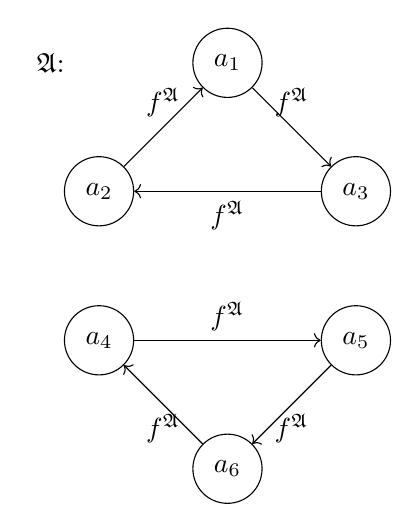
\begin{tikzpicture}
			\node[state] (a1) {$a_1$};
			\node[left=of a1, xshift=-0.5cm] (label) {$\mathfrak A$:};
			\node[state, below left=of a1] (a2) {$a_2$};
			\node[state, below right=of a1] (a3) {$a_3$};
			\node[state, below =of a2] (a4) {$a_4$};
			\node[state, below =of a3] (a5) {$a_5$};
			\node[state, below left=of a5] (a6) {$a_6$};
			\draw 
				(a1) edge[->, above] node{$f^{\mathfrak A}$} (a3)
				(a3) edge[->, below] node{$f^{\mathfrak A}$} (a2)
				(a2) edge[->, above] node{$f^{\mathfrak A}$} (a1)
				(a4) edge[->, above] node{$f^{\mathfrak A}$} (a5)
				(a5) edge[->, below] node{$f^{\mathfrak A}$} (a6)
				(a6) edge[->, below] node{$f^{\mathfrak A}$} (a4);
		\end{tikzpicture}
		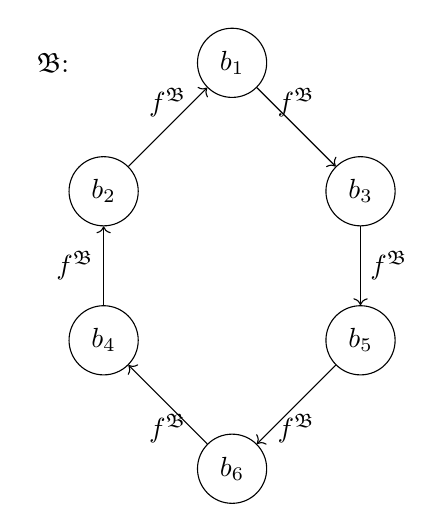
\begin{tikzpicture}
			\node[state] (b1) {$b_1$};
			\node[left=of b1, xshift=-0.5cm] (label) {$\mathfrak B$:};
			\node[state, below left=of b1] (b2) {$b_2$};
			\node[state, below right=of b1] (b3) {$b_3$};
			\node[state, below =of b2] (b4) {$b_4$};
			\node[state, below =of b3] (b5) {$b_5$};
			\node[state, below left=of b5] (b6) {$b_6$};
			\draw 
				(b1) edge[->, above] node{$f^{\mathfrak B}$} (b3)
				(b3) edge[->, right] node{$f^{\mathfrak B}$} (b5)
				(b5) edge[->, below] node{$f^{\mathfrak B}$} (b6)
				(b6) edge[->, below] node{$f^{\mathfrak B}$} (b4)
				(b4) edge[->, left] node{$f^{\mathfrak B}$} (b2)
				(b2) edge[->, above] node{$f^{\mathfrak B}$} (b1);
		\end{tikzpicture}
	\end{multicols}
	
	\caption{Two $\sigma$-structures $\mathfrak A$ and $\mathfrak B$}
	\label{NaiveEncodingCounterexample}
\end{figure}

Consider the formula $\phi=\exists x.(f(f(f(x)))=x)$ which utilizes term nesting to find a cycle with length three.
It is obvious that $\mathfrak A \models \phi$ and $\mathfrak B\not\models \phi$.
However, when encoding the two structures with the naive method described above, one finds that nRCR cannot distinguish them.
Therefore, term nesting is too powerful for the naive encoding.

A method that allows for the nesting of terms will be described in the following section.




\subsection{Using the transitive expansion} 
Let 
\begin{align*}
\mathcal I(n,m)=\{(k,l,p)\in [n]^3 \quad:\quad & k+p < k+l \leq n \; \land \\
& k+r\cdot l + p = m \text{ for some } r\in \mathbb N\}.
\end{align*}
The set will represents the possible ways, to decompose a path into a cycle and the path to and from it.
This means, that the triple $(k,\ell,p)$ will represent a path, that has a beginning part of length $k$, then a cycle of length $\ell$ and a last part that consists of the first $p$ elements of the cycle.
One can see that in a structure $\mathfrak A$ with a unary function $f$ and $n$ elements, any path along of $f$ with length $m>n$ can be decomposed into a triple in the set $\mathcal I(n,m)$.

\begin{lemma}
	Let $\psi(x_1,x_2)\coloneqq f^m(x_1)=x_2$. 
	Then there exists a formula $\theta(x_1,x_2)\in \GFC$ such that for any $\mathfrak A$ with $\Vert \mathfrak A\Vert=n$ it holds
	$$\mathfrak A,a_1,a_2 \models \psi(x_1,x_2) \text{ if, and only if, } \mathfrak A,a_1,a_2 \models \theta(x_1,x_2)$$ 
	and for any $f^{m'}(x)$ that appears in $\theta$, $m'\leq n$.
	\label{Simple_fm_to_fk}
\end{lemma}
\begin{proof}
	If $m \leq n$, we let $\theta\coloneqq\psi$ and the claim follows.
	
	Otherwise, we define
	$$\theta(x_1,x_2)\coloneqq \bigvee_{(k,\ell,p)\in \mathcal I(n,m)} \zeta_{(k,\ell,p)}(x_1,x_2)$$
	where
	\begin{align*}
		\zeta_{(k,\ell,p)}(x_1,x_2)\coloneqq & f^{k+p}(x_1)=x_2 \land f^{k}(x_1)=f^{k+\ell}(x_1) \\
		& \land \operatorname{E}^{k,\ell}_{f}(x_1)  \\
		& \land \bigwedge_{\ell'<\ell}f^{k}(x_1)\neq f^{k+\ell'}(x_1)
	\end{align*}
	and
	$$E^{k,\ell}_{f}(t(x_1))=\begin{cases}
		\top & \text{if } k=0 \\
		f^{k-1}(t(x_1))\neq f^{k-1+\ell}(t(x_1)) & \text{otherwise}.
	\end{cases}$$
	Due to the definition of $\mathcal I(n,m)$ it is obvious that only $f^{m'}$ with $m'\leq n$ appears.
	
	We now proceed to the proof of the equivalence.
	For the purpose of readability, we will use $f_{\mathfrak A}$ instead of $f^{\mathfrak A}$.
	
	We will show that if $\mathfrak A,a_1,a_2 \models \theta(x_1,x_2)$, then $\mathfrak A,a_1,a_2 \models \psi(x_1,x_2)$.
	Let $\mathfrak A,a_1,a_2 \models \theta(x_1,x_2)$. 
	By definition of $\theta$, there are $(k,\ell,p)\in \mathcal I(n,m)$ with $\mathfrak A,a_1,a_2 \models \zeta_{(k,\ell,p)}(x_1,x_2)$.
	In particular $f_{\mathfrak A}^{k}(a_1)=f_{\mathfrak A}^{k+\ell}(a_1)$. It follows that
	$$f_{\mathfrak A}^{k}(a_1)=f_{\mathfrak A}^{k+\ell}(a_1)=f_{\mathfrak A}^{k+2\ell}(a_1)=f_{\mathfrak A}^{k+3\ell}(a_1) = \dots = f_{\mathfrak A}^{k+r\cdot \ell}(a_1)$$
	for all $r\in \mathbb N$. By using the definition of $\mathcal{I}(n,m)$, we get
	$$a_2 =f_{\mathfrak A}^{k+p}(a_1) = f_{\mathfrak A}^{k+r\cdot \ell + p}(a_1)=f_{\mathfrak A}^{m}(a_1).$$
	From this we can deduce $\mathfrak A,a_1,a_2\models \psi(x_1,x_2)$, where $\psi(x_1,x_2)$ has the form $f^{m}(x_1)=x_2$.
	
	Now we prove that if $\mathfrak A,a_1,a_2 \models \psi(x_1,x_2)$, then $\mathfrak A,a_1,a_2 \models \theta(x_1,x_2)$. 
	Let $\mathfrak A,a_1,a_2\models \psi(x_1,x_2)$. By assumption $m>n$ and by the pigeonhole principle there have to be distinct $i, j$ such that $f_{\mathfrak A}^{i}(a_1)=f_{\mathfrak A}^{j}(a_1)$.
	Choose such $i$, $j$ such that they are lexicographically minimal.
	
	Now choose $k\coloneqq i$, $\ell \coloneqq j-i$ and $p\coloneqq (m-i) \mod (j-i)= (m-i) \mod \ell$.
	Obviously $(k,\ell,p)\in\mathcal I(n,m)$ and what remains to be shown is that $\mathfrak A,a_1,a_2\models \zeta_{(k,\ell,p)}(x_1,x_2)$.
	For that, we consider the parts of the conjunction and show for each one that it is satisfied.
	
	$f^{k+p}(x_1)=x_2$:
	We use the fact that $a= b \mod c \Leftrightarrow b = r\cdot c +a \text{ for some } r\in \mathbb N$.
	Then
	$$f_{\mathfrak A}^{k+p}(a_1)=f_{\mathfrak A}^{i+(m-i)-r\cdot \ell}(a_1)=f_{\mathfrak A}^{i+r\cdot \ell + m -i - r\cdot \ell}(a_1)=f_{\mathfrak A}^{m}(a_1)=a_2.$$
	Therefore $\mathfrak A,a_1,a_2\models f^{k+p}(x_1)=x_2$.
	
	$f^{k}(x_1)=f^{k+\ell}(x_1)$:
	Consider that
	$$f_{\mathfrak A}^{k}(a_1)=f_{\mathfrak A}^{i}(a_1)=f_{\mathfrak A}^{j}(a_1)=f_{\mathfrak A}^{j+i-i}(a_1)=f_{\mathfrak A}^{i+j-i}(a_1)=f_{\mathfrak A}^{k+\ell}(a_1).$$
	This leads to $\mathfrak A,a_1,a_2\models f^{k}(x_1)=f^{k+\ell}(x_1)$.
	
	$\operatorname{E}^{k,\ell}_f(x_1)$:
	This has to be satisfied, otherwise $f_{\mathfrak A}^{k-1}(a_1)=f_{\mathfrak A}^{k-1+\ell}(a)$, but then $(k-1,\ell)$ would be lexicographically smaller than $(i,j)$.
	
	The same reasoning applies to $\bigwedge_{\ell'<\ell}f^{k}(x_1)\neq f^{k+\ell'}(x_1)$. 
	If it weren't satisfied, there would be a $(i,j')$ with $j'<j$ and $f_{\mathfrak A}^{i}(a_1)=f_{\mathfrak A}^{i+j'}(a_1)$ which would be lexicographically smaller than $(i,j)$.
	
	Thus we have shown that every subformula of the conjunction and therefore the formula is being fulfilled.
\end{proof}

The above proof allows for the translation of formulae $f^m(x)=y$ to a formula $\theta(x,y)$ that is equivalent for structures with $n$ elements.
A natural extension would be, to allow alternation of functions, for example formulae like $g^m(f^{m'}(x))=y$.
This is also possible and will be proved in the following proof.

\begin{lemma}
	Let $\psi(x_1,x_2)\coloneqq t(x_1)=x_2$ be an atomic formula. 
	Then there exists a formula $\theta_{t}(x_1,x_2)\in\GFC$, such that for any structure (of a fitting signature) $\mathfrak A$ with $\Vert \mathfrak A \Vert = n$ it holds
	$$\mathfrak A,a_1,a_2 \models \psi(x_1,x_2) \text{ if, and only if, } \mathfrak A,a_1,a_2 \models \vartheta_{t}(x_1,x_2).$$ 
	Furthermore, $\theta_{t}(x_1,x_2)$ is of the form $\theta_{t}(x_1,x_2)=\bigvee \Phi(x_1,x_2)$ where all $\phi(x_1,x_2)\in\Phi(x_1,x_2)$ are of the form
	$$t'(x_1)=x_2 \land \bigwedge \Psi(x_1)$$ 
	for some term $t'(x_1)$, and for every $f^m(s(x))$ that appears in $\theta_{t}$, $m\leq n$.
\end{lemma}
\begin{proof}
	We prove this via an induction on the term $t(x_1)$.
	
	\textbf{Base case:}
	If $t(x_1)\coloneqq f^{m}(x_1)$ for a unary function symbol $f$ and $m\in \mathbb N$, we use the formula constructed in the proof of \cref{Simple_fm_to_fk}.
	It can easily be verified that it is in the correct form.
	
	\textbf{Inductive step:}
	Assume that $t(x_1)\coloneqq g^m(s(x_1))$ for a unary function symbol $g$, $m\in\mathbb N$ and term $s$.
	By induction hypothesis, we have a formula $\theta_{s}(y_1,y_2)=\bigvee \Phi_s(y_1,y_2)$ in the above defined form with $\mathfrak A,a_1,a_2 \models s(y_1)=y_2$ if, and only if, $\mathfrak A,a_1,a_2\models \theta_{s}(y_1,y_2)$.
	
	If $m\leq n$, we set 
	$$\theta_{t}(x_1,x_2)=\bigvee \Phi'(x_1,x_2),$$
	where $\Phi'(x_1,x_2)\coloneqq\{g^{m}(t'(y_1/x_1))=x_2 \land \bigwedge \Psi(y_1/x_1) : t'(y_1)=y_2 \land \bigwedge \Psi(y_1)\in \Phi_s(y_1,y_2)\}$.
	
	Now assume $m>n$.
	
	Then we set
	$$\theta_{t}(x_1,x_2)=\bigvee_{(k,\ell,p)\in \mathcal I(n,m)} \bigvee \Phi'_{(k,\ell,p)}(x_1,x_2),$$
	where 
	\begin{align*}
		\Phi'_{(k,\ell,p)}\coloneqq \{g^{k+p}(t'(y_1/x_1))=x_2 &\land g^{k}(t'(y_1/x_1))=g^{k+l}(t'(y_1/x_1)) \\
		& \land \operatorname{E}^{k,l}_g(t'(y_1/x_1)) \land \bigwedge_{\ell'<\ell} g^{k}(t'(y_1/x_1))\neq g^{k+\ell'}(t'(y_1/x_1)) \\
		& \land \Psi(y_1/x_1) : t'(y_1)=y_2 \land \bigwedge \Psi(y_1)\in \Phi_s(y_1,y_2)\}
	\end{align*}
	
	By using the above definitions, we get $\mathfrak A,a_1,a_2\models s(y_1)=y_2$ if, and only if, $\mathfrak A,a_1,a_2\models \phi_s(y_1,y_2)$ for some $\phi_s\in\Phi_s$ where $\phi_s(y_1,y_2)$ is of the form $t'(y_1)=y_2 \land \bigwedge \Psi(y_1)$.
	Therefore
	\begin{equation}
		\mathfrak A, a_1,a_2 \models s(y_1)=y_2 \text{ if, and only if, } \mathfrak A,a_1,a_2 \models t'(y_1)=y_2 \land \bigwedge \Psi(y_1).
		\label{Equivalence_s_and_tPsi}
	\end{equation}
	
	We now proof that 
	$$\mathfrak A, a_1,a_2\models t(x_1)=x_2 \text{ if, and only if, } \mathfrak A,a_1,a_2\models \theta_{t}(x_1,x_2).$$
	
	Assume $m\leq n$.
	Let $\mathfrak A, a_1,a_2 \models \theta_{t}$.
	Then there is some $\phi(x_1,x_2)\coloneqq g^{m}(t'(y_1/x_1))=x_2 \land \bigwedge \Psi(y_1/x_1)$ such that $\mathfrak A,a_1,a_2\models \phi(x_1,x_2)$.
	We then get
	\begin{align*}
		\mathfrak A,a_1,a_2 \models & g^{m}(t'(y_1/x_1))=x_2 \land \bigwedge \Psi(y_1/x_1) \\
		\Leftrightarrow \mathfrak A,a_1,a_2,a_3 \models & g^{m}(x_3)=x_2 \land \bigwedge \Psi(y_1/x_1) \land t'(y_1/x_1)=x_3 \text{ for all } a_3\in A \\
		\overset{\cref{Equivalence_s_and_tPsi}}{\Leftrightarrow} \mathfrak A,a_1,a_2,a_3\models & g^{m}(x_3)=x_2 \land s(x_1)=x_3 \text{ for all } a_3\in A \\
		\Leftrightarrow \mathfrak A,a_1,a_2 \models & g^{m}(s(x_1))=x_2.
	\end{align*}
	
	Now let $m>n$.
	Then there is a
	\begin{align*}
		\phi(x_1,x_2)\coloneqq g^{k+p}(t'(y_1/x_1))=x_2 &\land g^{k}(t'(y_1/x_1))=g^{k+l}(t'(y_1/x_1)) \\
		& \land \operatorname{E}^{k,l}_g(t'(y_1/x_1)) \land \bigwedge_{\ell'<\ell} g^{k}(t'(y_1/x_1))\neq g^{k+\ell'}(t'(y_1/x_1)) \\
		& \land \Psi(y_1/x_1)
	\end{align*}
	for some $(k,\ell,p)\in\mathcal I(n,m)$ with $\mathfrak A,a_1,a_2\models \phi(x_1,x_2)$.
	And now
	\begin{align*}
		\mathfrak A,a_1,a_2 \models & \psi(x_1,x_2) \\
		\Leftrightarrow A,a_1,a_2,a_3 \models &g^{k+p}(x_3)=x_2 \land g^{k}(x_3))=g^{k+l}(x_3) \\
			& \land \operatorname{E}^{k,l}_g(x_3) \land \bigwedge_{\ell'<\ell} g^{k}(x_3)\neq g^{k+\ell'}(x_3) \\
			& \land \Psi(y_1/x_1) \land t'(y_1/x_1)=x_3 \text{ for all } a_3\in A \\
		\overset{\cref{Simple_fm_to_fk}}{\Leftrightarrow} \mathfrak A, a_1,a_2,a_3 \models & g^{m}(x_3)=x_2 \land t'(y_1/x_1)=x_3 \land \Psi(y_1/x_1) \text{ for all } a_3 \in A \\
		\overset{\cref{Equivalence_s_and_tPsi}}{\Leftrightarrow} \mathfrak A,a_1,a_2,a_3 \models & g^{m}(x_3)=x_2\land s(x_1)=x_3 \text{ for any } a_3\in A \\
		\Leftrightarrow \mathfrak A,a_1,a_2 \models & g^{m}(s(x_1))=x_2.
	\end{align*}
	The other direction follows in both cases, as only equivalent steps have been used and it is obvious that the disjunction of a set is being fulfilled, if a formula of the set is satisfied.
	
	Therefore we have finished the proof.
\end{proof}

To obtain our characterising result for structures with (unary) functions, we have to define how the functions should be encoded.

\begin{definition}[Transitive Expansion]
	Let $\sigma\coloneqq \sigma_{\operatorname{Rel}} \operatorname{\dot{\cup}} \sigma_{\operatorname{Func}}$ be a signature with relation symbols $\sigma_{\operatorname{Rel}}$ and unary function symbols $\sigma_{\operatorname{Func}}$ and let $\mathfrak A$ be a structure of signature $\sigma$ with $\Vert \mathfrak A \Vert=n$.
	For readability, we define the family of sets $\operatorname{Alters}_n^0(\sigma)\coloneqq\emptyset$ and
	$$\operatorname{Alters}^k_{n}(\sigma)\coloneqq \operatorname{Alters}^{k-1}_{n}(\sigma)\cup\{f_1^{m_1}f_2^{m_2}\dots f_k^{m_k} : f_1f_2\dots f_k\in (\sigma_{\operatorname{Func}})^k, 0 \leq m_i \leq n \text{ for } 1 \leq i \leq k\}$$
	For an arbitrary $k\in \mathbb{N}$, we define the transitive expansion with alternation depth $k$ as a structure $\widetilde{\mathfrak A}$ of signature $\widetilde{\sigma}$, where 
	$$\widetilde{\sigma}\coloneqq \sigma_{\operatorname{Rel}} \operatorname{\dot{\cup}} \{F_\alpha : \alpha \in \operatorname{Alters}_n^k(\sigma)\}$$
	and the $F_\alpha$ are binary relations.
	Semantically, we have 
	$$F_\alpha^{\widetilde{\mathfrak A}}\coloneqq \{(a, b) : \alpha^{\mathfrak A}(a)=b\}.$$
\end{definition}

We now can define the algorithm for relational colour refinement for (unary) functions.

\begin{definition}[RCR for structures with unary functions]
	Let $\sigma$ be a signature with relation and unary function symbols and let $\mathfrak A$ and $\mathfrak B$ be structures of signature $\sigma$.
	
	We say that $\mathfrak A$ and $\mathfrak B$ are being distinguished by RCR with alternation depth $k$ ($\RCR_k$), if $\Vert\mathfrak A\Vert\neq \Vert \mathfrak B\Vert$ or the transitive expansions with alternation depth $k$, $\widetilde{\mathfrak A}$ and $\widetilde{\mathfrak B}$, are being distinguished by $\RCR$.
\end{definition}

To show that this definition may be sensible, we want to execute $\RCR_1$ on the structures $\mathfrak A$ and $\mathfrak B$ from \cref{NaiveEncodingCounterexample}.
First we compute $\widetilde\sigma$ as $\{F_{f^i} : 0\leq i \leq 6\}$ and by performing the translation we obtain:
\begin{align*}
	\widetilde{\mathfrak A}=(A, 
	&F_{f^0}^{\widetilde{\mathfrak A}}=\{(a_1, a_1), (a_2, a_2),(a_3, a_3), (a_4, a_4), (a_5, a_5), (a_6, a_6)\}, \\
	&F_{f^1}^{\widetilde{\mathfrak A}}=\{(a_1, a_3), (a_2, a_1),(a_3, a_2), (a_4, a_5), (a_5, a_6), (a_6, a_4)\}, \\
	&F_{f^2}^{\widetilde{\mathfrak A}}=\{(a_1, a_2), (a_2, a_3),(a_3, a_1), (a_4, a_6), (a_5, a_4), (a_6, a_5)\}, \\
	&F_{f^3}^{\widetilde{\mathfrak A}}=\{(a_1, a_1), (a_2, a_2),(a_3, a_3), (a_4, a_4), (a_5, a_5), (a_6, a_6)\}, \\
	&F_{f^4}^{\widetilde{\mathfrak A}}=\{(a_1, a_3), (a_2, a_1),(a_3, a_2), (a_4, a_5), (a_5, a_6), (a_6, a_4)\}, \\
	&F_{f^5}^{\widetilde{\mathfrak A}}=\{(a_1, a_2), (a_2, a_3),(a_3, a_1), (a_4, a_6), (a_5, a_4), (a_6, a_5)\}, \\
	&F_{f^6}^{\widetilde{\mathfrak A}}=\{(a_1, a_1), (a_2, a_2),(a_3, a_3), (a_4, a_4), (a_5, a_5), (a_6, a_6)\})
\end{align*}
and 
\begin{align*}
	\widetilde{\mathfrak B}=(B, 
	&F_{f^0}^{\widetilde{\mathfrak B}}=\{(a_1, a_1), (a_2, a_2),(a_3, a_3), (a_4, a_4), (a_5, a_5), (a_6, a_6)\}, \\
	&F_{f^1}^{\widetilde{\mathfrak B}}=\{(a_1, a_3), (a_2, a_1),(a_3, a_5), (a_4, a_2), (a_5, a_6), (a_6, a_4)\}, \\
	&F_{f^2}^{\widetilde{\mathfrak B}}=\{(a_1, a_5), (a_2, a_3),(a_3, a_6), (a_4, a_1), (a_5, a_4), (a_6, a_2)\}, \\
	&F_{f^3}^{\widetilde{\mathfrak B}}=\{(a_1, a_6), (a_2, a_5),(a_3, a_4), (a_4, a_3), (a_5, a_2), (a_6, a_1)\}, \\
	&F_{f^4}^{\widetilde{\mathfrak B}}=\{(a_1, a_4), (a_2, a_6),(a_3, a_2), (a_4, a_5), (a_5, a_1), (a_6, a_3)\}, \\
	&F_{f^5}^{\widetilde{\mathfrak B}}=\{(a_1, a_2), (a_2, a_4),(a_3, a_1), (a_4, a_6), (a_5, a_3), (a_6, a_5)\}, \\
	&F_{f^6}^{\widetilde{\mathfrak B}}=\{(a_1, a_1), (a_2, a_2),(a_3, a_3), (a_4, a_4), (a_5, a_5), (a_6, a_6)\})
\end{align*}

By using \cite{scheidt2025ColorRefinement}, we know that $\RCR$ distinguishes $\widetilde{\mathfrak A}$ and $\widetilde{\mathfrak B}$ if, and only if, there is a formula $\widetilde{\phi}\in\GFC$ of signature $\widetilde{\sigma}$ that distinguishes them.
Notice that $F_{f^0}^{\widetilde{\mathfrak A}}=F_{f^3}^{\widetilde{\mathfrak A}}=F_{f^6}^{\widetilde{\mathfrak A}}$, $F_{f^1}^{\widetilde{\mathfrak A}}=F_{f^4}^{\widetilde{\mathfrak A}}$ and $F_{f^2}^{\widetilde{\mathfrak A}}=F_{f^5}^{\widetilde{\mathfrak A}}$, while only $F_{f^0}^{\widetilde{\mathfrak B}}=F_{f^6}^{\widetilde{\mathfrak B}}$.
Therefore the sentence 
$$\exists^{\geq 6}(x,y).\left(F_{f^1}(x,y) \land F_{f^4}(x,y)\right)\in \GFC$$ 
is satisfied by $\widetilde{\mathfrak A}$, but not $\widetilde{\mathfrak B}$.

We see, that this procedure distinguishes structures, that were not distinguished by nRCR.
To formalise this, we want to characterise this algorithm logically, as well as combinatorially.

\subsubsection{Logical characterisation of $\RCR_k$}

\begin{definition}[Alternation bounded $\GFC$]
	The fragment of $\GFC$ with an alternation bound of $k$ ($\GFC_k$) is $\GFC$ with the constraint that for all formulae $\phi\in\GFC_k$ of signature $\sigma$ and every term $t$ that appears in $\phi$, there is an $n\in \mathbb{N}$ and an $\alpha\in \operatorname{Alters}_n^k(\sigma)$ such that $\alpha=t$.
	Atomic formulae are defined as usual, that is, the formulae $R(t_1(x_1),t_2(x_2),\dots,t_n(x_n))$ and $t_1(x_1)=t_2(x_2)$ for terms $t_1,t_2,\dots,t_n$ and variables $x_1,x_2,\dots,x_n$ are atomic formulae.
\end{definition}

\begin{theorem}
	Let $\mathfrak A$ and $\mathfrak B$ be two structures of the same signature $\sigma$ with relation and unary function symbols and let $k\in \mathbb{N}$
	The two following statements are equivalent:
	\begin{enumerate}
		\item $\RCR_k$ distinguishes $\mathfrak A$ and $\mathfrak B$.
		\item There exists a sentence $\phi\in\GFC_k$ such that $\mathfrak A\models \phi$ and $\mathfrak B\not\models \phi$.
	\end{enumerate}
\end{theorem}
\begin{proof}
	We prove that \emph{1.} implies \emph{2.}. 
	Let $\mathfrak A$ and $\mathfrak B$ be distinguished by $\RCR_k$.
	If they are of different sizes, assume without loss of generality that 
	$$\Vert \mathfrak A \Vert =n > n'=\Vert \mathfrak B \Vert.$$
	Then define $\phi\coloneqq \exists^{\geq n} x. \top\in \GFC_k$, which obviously distinguishes the structures.
	
	Now assume $\Vert \mathfrak A\Vert = \Vert \mathfrak B \Vert = n$.
	By definition, $\RCR$ distinguishes $\widetilde{\mathfrak A}$ and $\widetilde{\mathfrak B}$.
	When using the proof from \cite{scheidt2025ColorRefinement}, we obtain a formula $\widetilde{\phi}\in \GFC$ of signature $\widetilde{\sigma}$ that distinguishes the expansions.
	This formula $\widetilde{\phi}$ can then be translated to a formula $\phi\in\GFC_k$ of signature $\sigma$.
	
	For every atomic subformula $R(\mathbf x)$, where $R\in \sigma_{\operatorname{Rel}}$, let the formula stay the same.
	For every atomic subformla $F_\alpha(x,y)$, where $\alpha\in \operatorname{Alters}_n^k(\sigma)$, replace it by the formula $\alpha(x)=y$. Obviously, if a structure's expansion satisfied $\widetilde{\phi}$, it also satisfies $\phi$ and vice versa.
	
	Therefore, we get a formula $\phi\in \GFC_k$ that distinguishes $\mathfrak A$ and $\mathfrak B$.
	\break
	Now we prove that \emph{2.} implies \emph{1.}.
	Let $\phi\in \GFC_k$ such that $\mathfrak A\models \phi$ and $\mathfrak B\not\models \phi$.
	
\end{proof}

% Now:
% 	- Proof that if theta is satisfied, exactly one subformula of the conjunction is satisfied
%		- Use this to permute \exists>=n \bigvee Phi to get \bigvee \exists>=n Phi -> Use Delta as guard
%		- Allows usage of terms with higher nesting numbers than n as guards
%	- Proof sketch for atomics of the form t(x_1)=s(x_2)
%		- Should be pretty simple by using the last proof to widen formula to y_1=y_2 and t(x_1)=y_1 and s(x_2)=y_2; Then apply proof and resubstitute


\section {Relational Colour Refinement for symmetric structures}

\lipsum[3-4]

\section{Conclusion}

\lipsum[2-3]


\clearpage

\bibliographystyle{plainurl}
\bibliography{references.bib}





\end{document}





